Um zu überprüfen, ob bestimmte partielle Sudokus eindeutig lösbar sind, haben wir uns verschiedene Lösungsmöglichkeiten überlegt.
Die zwei wichtigsten Überlegungen waren ein CSP-Solver (Constraint Satisfaction Problem) oder ein SAT-Solver (Satisfiability).
Um herauszufinden, welcher dieser Ansätze eine schnellere Lösung bietet, haben wir ein Python-Skript geschrieben, welches diesen Sachverhalt untersuchen sollte~\cite{sat_csp_comparison}.

Dafür musste das Problem für die Löser umformuliert werden, einmal musste ein Sudoku also als Constraints und Dimensionen für den CSP-Solver formuliert werden. 
Und zweitens muss man Sudoku auf SAT reduzieren.

\begin{enumerate}
    \item CSP-Solver \\
    Das Sudoku lässt sich elegant als CSP darstellen. Dafür betrachten wir das Spielfeld als Menge
    $$
        X = \{x_{i,j}|1 \leq i,j \leq n\}
    $$
    Jede Variable $x_{i,j}$ kriegt hier also eine Domäne von Werten die gegeben ist durch $D(x_{i,j}) = \{1, 2, \dots, n$\}. 
    Zuletzt müssen noch die Constraints angegeben werden.
    Für jede Zelle $z_{i, k}$ einer Reihe, dass $x_{i, k} \neq x_{j, k}$ mit $j \neq i$.
    Das Gleiche gilt für die Spalten, also $x_{i, k} \neq x_{i, l}$ mit $k \neq l$, und auch für die Untergitter.
    Die Hinweise eines Sudokus werden auch als Constraints gegeben. Wenn z.B. in der ersten Spalte und in der ersten Zeile eine 5 steht dann wäre die Variable $D(x_{1, 1}) = \{5\}$.
    
    %Um das Problem eines Sudokus in ein CSP zu übertragen haben wir schlicht die Domänen der Zellen auf die Werte $1, 2, \dots, 9$ gesetzt 
    %und die Sudoku Regeln jeweils in Constraints übersetzt und anschließend die Domänen der schon vorgegebenen Zellen nur auf die eingegebenen Zahlen eingeschränkt.
    %Die Constraints waren also für jede Zelle $z_{i, k}$ einer Reihe, dass $z_{i, k} \neq z_{j, k}$ mit $j \neq i$.
    %Das Gleiche gilt für die Spalten, also $z_{i, k} \neq z_{i, l}$ mit $k \neq l$.
    %Für die Unterquadrate wurden jeweils auch wieder geprüft, dass jede Zelle nicht den gleichen Wert haben darf wie eine andere im Unterquadrat.

    \item SAT-Solver \\
    Um Sudokus auf SAT zu reduzieren müssen wir erst alle Variablen als Wahrheitswerte darstellen. Wir haben also eine Formel benutzt die jeder Kombination an Reihe, Spalte und jedem Wert einen einheitlichen Wahrheitswert zuweist.
    \begin{equation}
        V(r, c, d) = n^2 \cdot (r - 1) + n \cdot (c - 1) + d
    \end{equation}
    Weiter müssen wir jetzt das Sudoku als konjunktive Normalform darstellen. 
    Als erstes mussten wir festlegen, dass jede Zelle mindestens eine Zahl enthält, was mit dieser Menge an Klauseln dargestellt wurde:
    \begin{equation}
        \forall i, j, k: V(i, j, k) \text{ mit } i, j, k \in \{1, ..., n\} %TODO Werte und Reihen/Spalten gleiche Menge?
    \end{equation}
    und, dass jede Zelle maximal eine Zahl enthält, wiederum mit dieser Menge an Klauseln.
    \begin{equation}
        \forall i, j, k_1, k_2: \neg V(i, j, k_1) \vee \neg V(i, j, k_2) \text{ mit }i, j, k_1, k_2 \in \{1, ..., n\} \text{ und } k_1 \neq k_2 %TODO auf generelle größe anpassen?
    \end{equation}
    Des weiteren musste nun für jede Reihe, jede Spalte und jedes Untergitter bestimmt werden, dass zwei Zellen nicht den gleichen Wert und alle Werte $1, \dots, n$ %TODO auf generelle größe anpassen?
    in der Zeile, Spalte oder dem Untergitter enthalten sein müssen.
    Das funktioniert gleich wie bei den Regeln für das ganze Sudoku nur das die $i, j$ Werte entweder auf die Reihe, die Spalte oder das Untergitter beschränkt ist.
    Wir verunden also anschließend alle Kaluseln die wir erstellt haben, dadurch kann der SAT-Solver sie nun lösen.
    Um die Hinweise hinzuzufügen, nimmt man also nun an, dass bestimmt Variablen wahr sind und löst dann mit dieser Annahme das SAT-Problem.
\end{enumerate}

Um die Lösungsansätze miteinander vergleichen zu können, haben wir jeweils 100 4x4, 6x6 und 9x9 Sudokus lösen lassen.
Hierfür haben wir einmal den cadical SAT-Solver~\cite{pysat} verwendet und außerdem die verschiedenen Solver einer CSP-Solver library~\cite{pycsp}.
Wir haben einmal den Durchschnitt der Zeiten pro Solver für das reine Lösen ausgewertet und die Anzahl der abgelaufenen Durchläufe, also die Durchläufe die über eine Sekunde gedauert haben.

    \begin{figure*}[t]
        \centering
        
        \begin{subfigure}[b]{0.8\textwidth}
            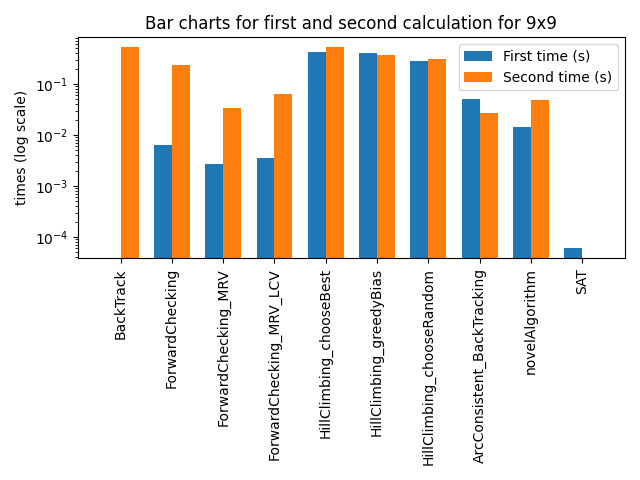
\includegraphics[width=\textwidth]{data/times_9x9}
            \caption{times 9x9}
        \end{subfigure}
        \hfill
        \begin{subfigure}[b]{0.8\textwidth}
            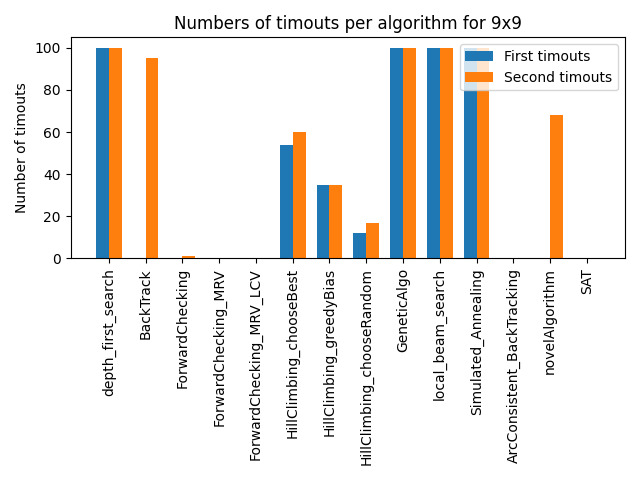
\includegraphics[width=\linewidth]{data/timeouts_9x9}
            \caption{timeouts 9x9}
        \end{subfigure}
        
        \caption{Comparison of times and timeouts for different solving Algorithms}
    \end{figure*}

Wie man unschwer erkennen kann, ist der SAT-Solver mit Abstand am schnellsten und löst die Sudokus innerhalb von meist nicht messbarer Zeit. 
Genau gleich sieht es mit den Timeouts aus, bei allen 100 Sudokus hat der SAT-Solver alle Lösungen gefunden. Viele der anderen Solver haben keine einzige Lösung in der gegebenen Zeit gefunden.
Auch wenn sich manche CSP-Lösungsverfahren gut gehalten haben, macht es keinen Sinn etwas anderes als den getesteten SAT-Solver zu verwenden.
Wir können mit ähnlicher Performanz rechnen, da auch cadical-rs so wie die Implementierung in Python auf ersichtlich schnellem Code in C/C++ laufen.
